% Full instructions available at:
% https://github.com/elauksap/focus-beamertheme

\documentclass[9pt]{beamer}
\usetheme{focus}

%%%%%%%%%%%%%%%%%%%%%%%%%%%%%%%%%%%%%%%%%%%%%%%%%%%%%%%%%%%%%%%%%%%%%
% Typography, change document font
\usepackage[tt=false, type1=true]{libertine}
\usepackage[varqu]{zi4}
\usepackage[libertine]{newtxmath}
\usepackage[T1]{fontenc}

\usepackage[protrusion=true,expansion=true]{microtype}

% Disable paragraph indentation, and increase gap
\usepackage{parskip}

%Matrix
\usepackage{tabstackengine}
\setstackEOL{;}% row separator
\setstackTAB{,}% column separator
\setstacktabbedgap{1ex}% inter-column gap 
\setstackgap{L}{1.0\normalbaselineskip}% inter-row baselineskip
\let\mat\bracketMatrixstack

\newcommand{\pth}{Figure/}
\newcommand{\ve}[1]{\mathbf{#1}}

% Copyright (C) 2018-2019 Pasquale Claudio Africa and the LaTeX community.
% A full list of contributors can be found at
%
%     https://github.com/elauksap/focus-beamertheme
% 
% This file is part of beamerthemefocus.
% 
% beamerthemefocus is free software: you can redistribute it and/or modify
% it under the terms of the GNU General Public License as published by
% the Free Software Foundation, either version 3 of the License, or
% (at your option) any later version.
% 
% beamerthemefocus is distributed in the hope that it will be useful,
% but WITHOUT ANY WARRANTY; without even the implied warranty of
% MERCHANTABILITY or FITNESS FOR A PARTICULAR PURPOSE. See the
% GNU General Public License for more details.
% 
% You should have received a copy of the GNU General Public License
% along with beamerthemefocus. If not, see <http://www.gnu.org/licenses/>.

\mode<presentation>


% DEFINE COLORS. ---------------------------------------------------------------
\definecolor{main}{RGB}{134, 161, 174}
\definecolor{main2}{RGB}{104, 131, 144}
\definecolor{textc}{RGB}{20, 20, 20}
\definecolor{background}{RGB}{255, 255, 255}

\definecolor{alert}{RGB}{180, 0, 0}
\definecolor{example}{RGB}{0, 110, 0}


% SET COLORS. ------------------------------------------------------------------
\setbeamercolor{normal text}{fg=textc, bg=background}
\setbeamercolor{alerted text}{fg=textc}
\setbeamercolor{example text}{fg=textc}

\setbeamercolor{titlelike}{fg=background, bg=main}
\setbeamercolor{frametitle}{parent={titlelike}}

\setbeamercolor{footline}{fg=background, bg=main2}

\setbeamercolor{block title}{bg=main!80!background, fg=background}
\setbeamercolor{block body}{bg=main!10!background, fg=textc}

\setbeamercolor{block title alerted}{bg=alert, fg=background}
\setbeamercolor{block body alerted}{bg=alert!10!background, fg=textc}

\setbeamercolor{block title example}{bg=example, fg=background}
\setbeamercolor{block body example}{bg=example!10!background, fg=textc}

\setbeamercolor{itemize item}{fg=textc}
\setbeamercolor{itemize subitem}{fg=textc}

\setbeamercolor{enumerate item}{fg=textc!70!black}
\setbeamercolor{enumerate subitem}{fg=textc!70!black}

\setbeamercolor{description item}{fg=textc!70!black}
\setbeamercolor{description subitem}{fg=textc!70!black}

\setbeamercolor{caption name}{fg=textc}

\setbeamercolor{section in toc}{fg=textc}
\setbeamercolor{subsection in toc}{fg=textc}
\setbeamercolor{section number projected}{bg=textc}
\setbeamercolor{subsection number projected}{bg=textc}

\setbeamercolor{bibliography item}{fg=main}
\setbeamercolor{bibliography entry author}{fg=main!70!black}
\setbeamercolor{bibliography entry title}{fg=main}
\setbeamercolor{bibliography entry location}{fg=main}
\setbeamercolor{bibliography entry note}{fg=main}

\mode<all>


\begin{document}
	\tableofcontents

\section{Tangent matrix : \today}
	\begin{frame}{Introduction}
		\begin{itemize}
			\item Linearity allows us to know the solution at any value. What I mean is if we have a function f(x), we can find the slope at any point of f and then get the solution
			\item In nonlinear cases, the slope at one point may not represent the actual solution at another so we have an issue. So we linearise the solution at some point and then find how far off is the linear solution from the nonlinear one. 
			\item We will focus here on different derivations of the tangent stiffness matrix for different domains	
		\end{itemize}
	\end{frame}
		
\section{Euler beam elements}		
	\begin{frame}{Beam elements}
		\begin{itemize}
			\item For the euler beam element we get the stiffness matrix as follows  \\
			$\mat{K^{11},K^{12} ; K^{21},K^{22}} \mat{\Delta^1 ; \Delta^2} = \mat{F^1 ; F^2}$
			where we see a coupling between the two dof here (Note there are more dof inside each one)
			\item Sometimes we can derive the stiffness matrix terms involving the von karman nonlinearity $ \frac{\partial dw}{\partial dx}$ insuch a way that $K^{12}$ = 0 and so the nonlinear equations become uncoupled and we can solve them iteratively. In this case u and w will become nonlinear terms. 
			However the tangent matrix will remain the same.
		\end{itemize}
	\end{frame}	

	\begin{frame}{Iterative strategies}
		\begin{itemize}
			\item In direct method, we just keep looping through the process till the nonlinear terms or the residual stabilise.
			\item Here we talk about the NR method:
			\item There are two things which are a bit complicated. One is the position of a body and the other is the displacement whereby it moves towards the equilibrium state.
			\item We see from the directional derivative notes, that the directional derivative is used to linearise two things, one is the functional of the potential energy which gives us our equilibrium equations
			\item The other linearisation is of these equilibrium equations giving us a linearised version of the equations at a location.		
		\end{itemize}

	\end{frame}


	\begin{frame}
		\begin{itemize}
			\item The main problem lies I guess in the assumption of small deformations. FIX ME!!!!!!!!!!!!!!!!!!!
			\item We have a functional which is has both internal and external work . $\Pi = d^TKd - Fd$
			\item This energy functional is therefore dependant on the intial undeformed geometry. Based on it if we move by some displacement d, we change the internal energy and potential of the external work.
			\item In the Updated weight method, we however keep the energy in terms of the location in space. Once we found the first directional derivative, invariably we became intersted in displacements. But these displacements were of an energy functional that depended only on the position. 
			\item What is then the difference between $du$ and $dx$??? I think that u is the way to think about it.
			\item The first directional derivative gives you the direction that you need to move your displacement such that your potential energy gets minimized. Again note that the potential is ususally referenced to an undeformed shape. 
		\end{itemize}
	\end{frame}

	\begin{frame}{NR method}
		\begin{itemize}
			\item We have the residual equation given as 
			$\ve{R = F - K }\Delta$
			\item Linearising this we get $\ve{R^{i+1} = R^i +} \frac{d R}{d  \Delta}|_i \delta \Delta$ \\
			Interesting thing to note is that the derivative of the residual is with respect to the displacements, and the small amount we move is in a small direction in that displacement we're actually on. That is the displacement increment !!! $\Delta U$ 
			
			\begin{figure}
				\centering
				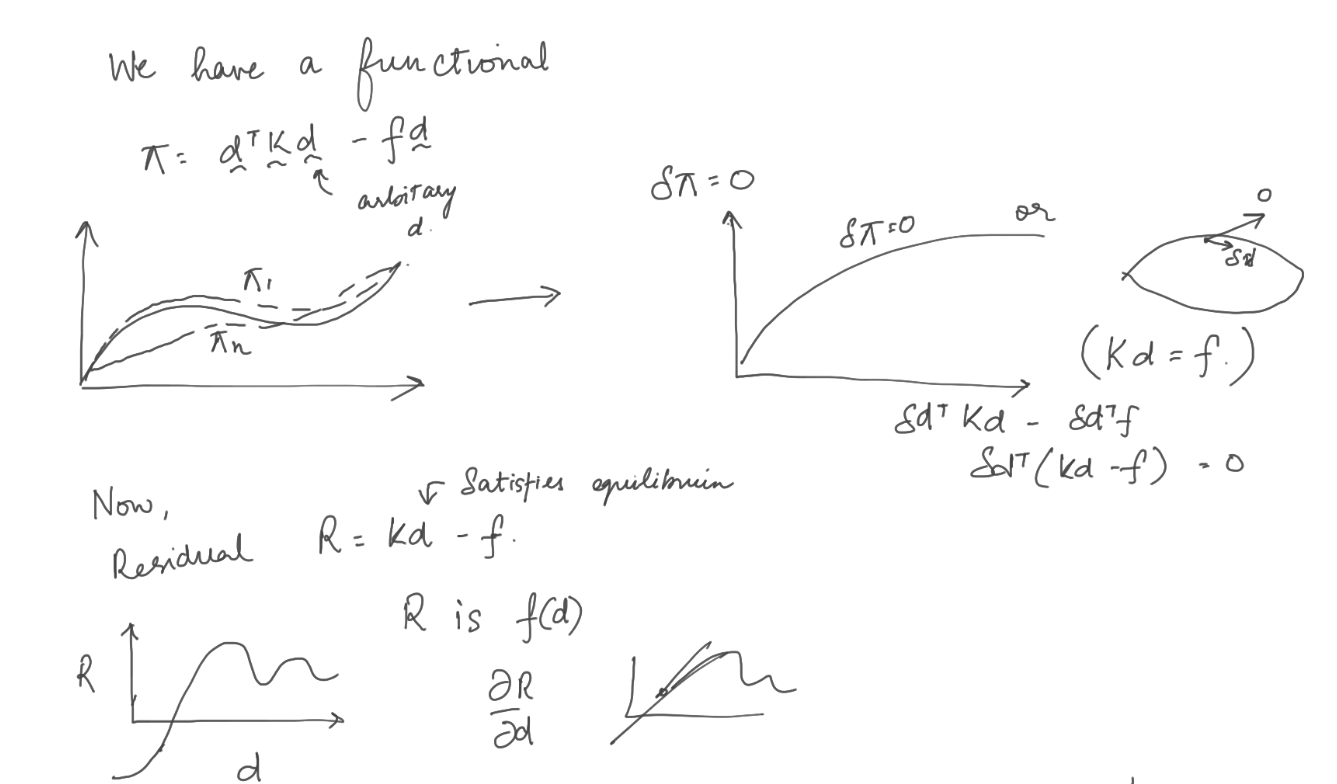
\includegraphics[width=0.7\linewidth]{Figure/1}
				\caption{}
				\label{fig:1}
			\end{figure}
		\end{itemize}
	\end{frame}


	\begin{frame}
		\begin{itemize}
			\item In Reddy 5.2.43 we get our displacement increment, which is $\Delta U = -\left( T(U^{r-1}) \right)^{-1} R^{r-1}$ 
			\item Where the next solution is then found as $\ve{U^{r} = U^{r-1}+ } \Delta \ve{U}$
			\item The coefficients of the tangent stiffness amtrix has a similar structure to $\ve{K}$ so we can have the form
			$\mat{T^{11},T^{12} ; T^{21},T^{22}} \mat{\delta \Delta^1 ; \delta \Delta^2} = - \mat{R^1 ; R^2}$
			\item Note that each coeffcients in both $\ve{T}$ and $ \Delta$ are matrices and vectors.
			\item So lets say that $T^{11} \delta \Delta^{1} + T^{12} \delta \Delta^{2} =  - R^{1}$  or  \\
			$T^{11}_{ij} \delta \Delta^{1}_j + T^{12}_{ij} \delta \Delta^{2}_j =  - R^{1}_i$
			\item Here we note that each component of T and $\Delta$ are matrices.		\end{itemize}
	\end{frame}

	\begin{frame}
		% TODO: \usepackage{graphicx} required
		\begin{figure}
			\centering
			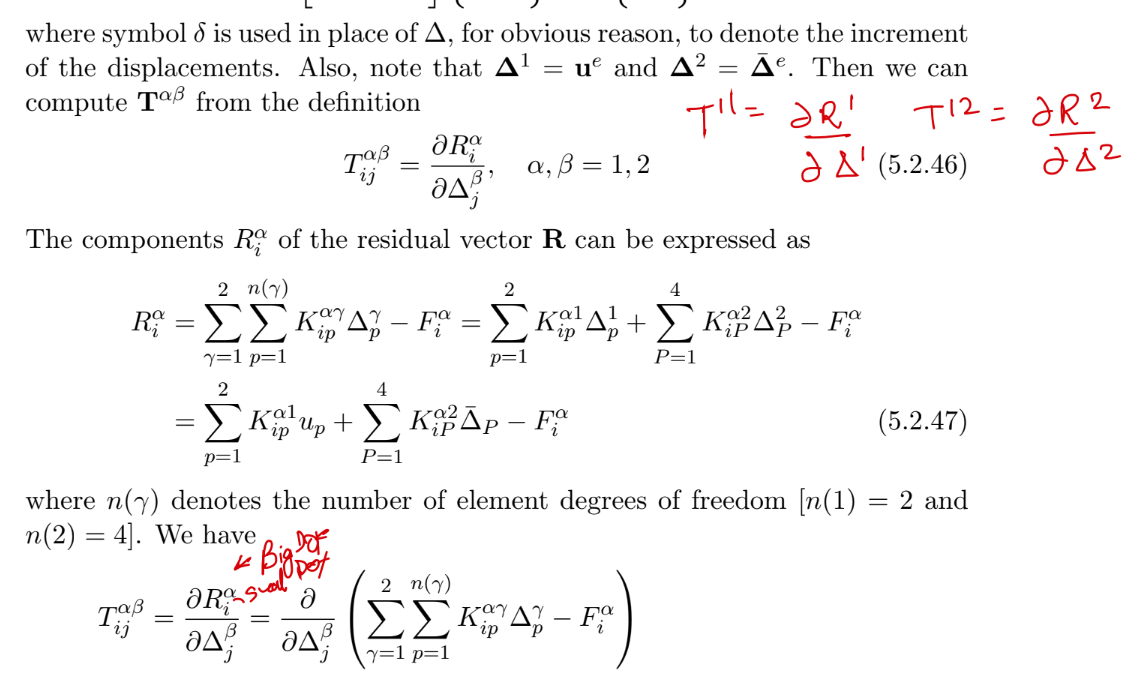
\includegraphics[width=0.8\linewidth]{Figure/2}
			\label{fig:2}
		\end{figure}
		\begin{itemize}
			\item Here we see that the top indices are for the smaller condensed matrix while the lower one takes care of every degree of freedom. 
			\item Note that $n(\gamma)$ means the summation differs depending on whether its u(2 dof per node ) and $\bar{\Delta}$ having 4 dof per node. 
			\item Pretty interesting
		\end{itemize}
	\end{frame}


	\begin{frame}
		\begin{figure}
			\centering
			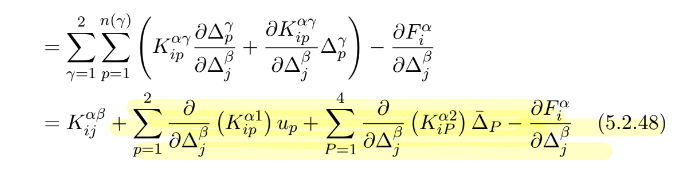
\includegraphics[width=0.8\linewidth]{Figure/3}
			\label{fig:3}
		\end{figure}
		\begin{itemize}
			\item We get the tangent matrix as above. 
			\item Since the derivative is not summed, we can take it inside for every summation of $\gamma, p, \alpha$ 
			\item Since $\beta, j$ are not summed over, we get our $K^{\alpha \beta}_{ij}$ out. The other terms are the actuall summed terms of the condensed dof $\gamma$ and because of that each $\gamma$ dof corresponds to the actual one of u(p=2) or $\bar{\Delta }$ (p=4)

			
		\end{itemize}
	\end{frame}


	\begin{frame}{Tangent components}
		\begin{itemize}
			\item In finding the tangent stiffness components, the stiffness components have to be recalled. 
			% TODO: \usepackage{graphicx} required
			\begin{figure}
				\centering
				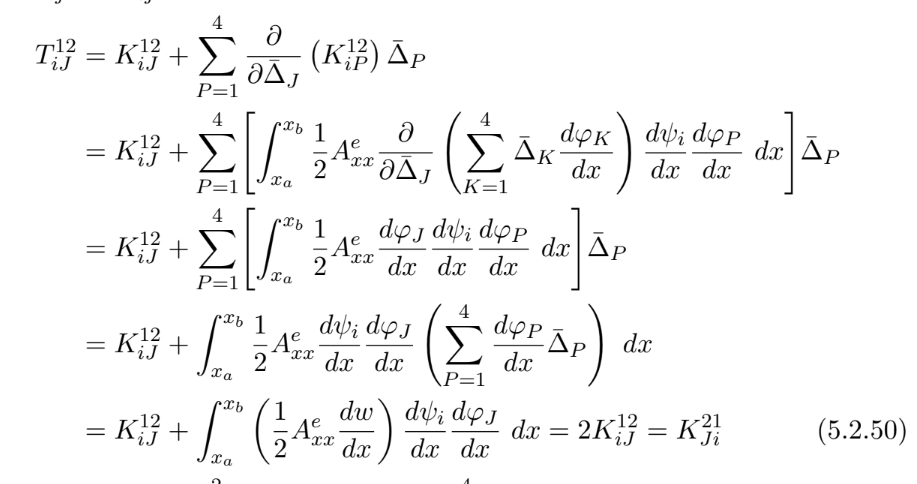
\includegraphics[width=0.7\linewidth]{Figure/4}
				\label{fig:4}
			\end{figure}
			\item $T^{12}$ is for the coupling of the membrane and bending dof. Now we know that it's rate of change of membrane residual by the bending dof. For each row $i$ of the dof p, we see that term due to u is 0 as the derivative is $\bar{\Delta}$. In the stiffness term, note that the nonlienar term is $\frac{dw}{dx} = \sum \bar{\Delta} \frac{d \phi}{dx}$ which is getting differentiated.
		\end{itemize}
	\end{frame}


	\begin{frame}
		\begin{itemize}
			\item % TODO: \usepackage{graphicx} required
			\begin{figure}
				\centering
				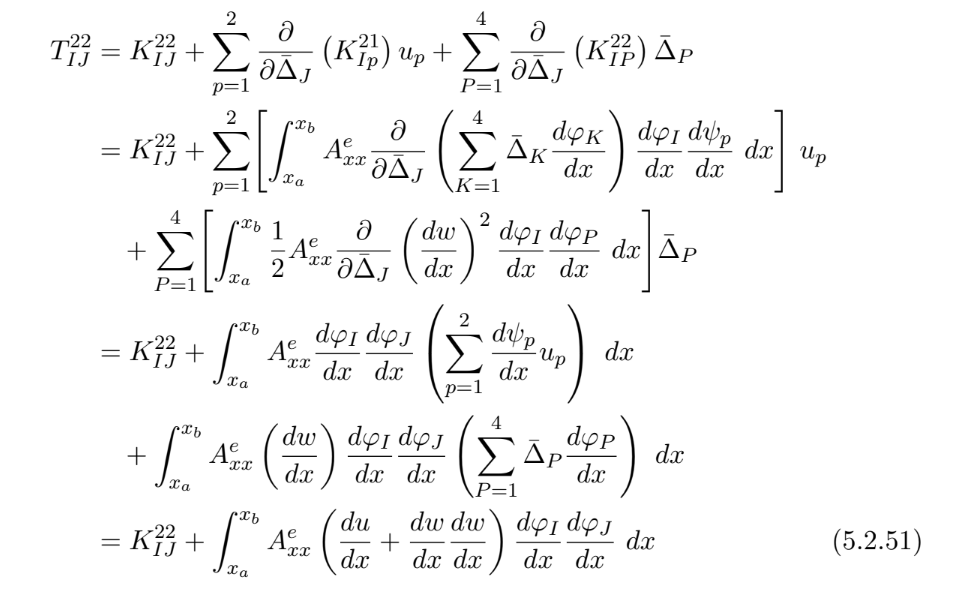
\includegraphics[width=0.7\linewidth]{Figure/5}
				\label{fig:5}
			\end{figure}
			 \item For $T^{22}$, all the dof are included. Interesting!
			
		\end{itemize}
	\end{frame}


\section{Plates}


	\begin{frame}
		
	\end{frame}

\end{document}